\documentclass[border=8pt]{standalone}
\usepackage[utf8]{inputenc}
\usepackage{tikz}
\tikzset{
  debole/.style = {rectangle, draw, thick, fill=blue!8, double, double distance=1.5pt, minimum width=26mm, minimum height=14mm, font=\small},
  attr/.style   = {circle, draw, thick, fill=white, minimum size=5pt, inner sep=0},
  link/.style   = {thick}, et/.style = {font=\footnotesize}
}
\begin{document}
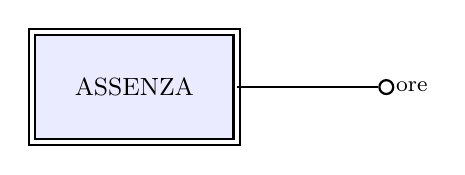
\begin{tikzpicture}
  % identificazione esterna: giorno + causale
  \node[debole] (E) {ASSENZA};
  \node[attr] (o) at (3.2,0){}; \draw[link] (1.3,0)--(o); \node[et,right] at (o) {ore};
\end{tikzpicture}
\end{document}
